In Chapter 1, we introduce a two-stage rolling-horizon re-planning simulation framework. Using this framework and a realistic test dataset, we simulate \emph{status quo} interaction between the principal (i.e., government steward of Crown forest) and the agent (i.e., industrial fibre consumer). We conclude Chapter 1 by observing that the classic wood supply optimization model formulation does not predict wood supply failures under certain circumstances\footnote{Specifically, the classic wood supply model fails to predict wood supply failures when industrial fibre consumption is a species-skewed subset of AAC.}, and conjecture that risk of wood supply failures could be mitigated by extending the classic wood supply model to explicitly anticipate industrial fibre consumption behaviour.

In Chapter 2, we present a bilevel wood supply model formulation that anticipates fibre consumption, and develop a solution algorithm to solve a special case of the problem to global optimality. We compare performance of classic and bilevel wood supply models using the simulation framework and test dataset introduced in Chapter 1. We conclude that the bilevel model successfully mitigates risk of wood supply failure, although there is some residual instability in long-term wood supply. 

Note that for our case study test dataset, we simulate a tension between hardwood and softwood fibre consumption. Although the simulation results presented here cannot be directly generalized to other cases, our rolling-horizon simulation framework and bilevel modelling methodology could potentially provide valuable insight into long-term sustainability of wood supply for a range of common problem instances. For example, some areas are characterised by asymmetrical industrial demand between spruce and fir\footnote{Spruce tends to be more highly valued as a raw material for lumber than fir, primarily due to longer kiln-drying times required to produce fir lumber with the targeted final moisture content.}, which would induce principal-agent problems similar to the one described in our case study.

In this chapter, we explore sensitivity of long-term wood supply to various simulation parameters. Using our two-stage rolling-horizon re-planning simulation framework, each scenario simulates 30 planning cycles. Scenarios are grouped into five series, with each series testing different levels of a given parameter. 

All simulation results presented in this chapter use the test dataset described in Chapter 1. Unless specified otherwise, all scenarios use the bilevel model to determine wood supply at each planning cycle and simulate perfect anticipation of agent fibre consumption volume. 

The reference scenario for all series is the base bilevel scenario\footnote{For the reference scenario, the principal uses the bilevel model to determine AAC, and the agent is allowed to replan harvesting on a one-period horizon, choosing the profit-maximizing subset of available wood supply. Due to the optimal formulation of the bilevel model and perfect anticipation of volume consumption, the agent always chooses to harvest the entire wood supply. However, the agent may select to harvest this volume from a different combination of forest types than what was prescribed in the first period of the principal’s optimal solution.}, which we first introduced as Scenario 3 in Chapter 2 (see \S\ref{sec:experimental_methodology2}). We include the reference scenario in all scenario series, and specify where it can be found in each sequence (it changes position and name, depending on the context).  

We present simulation results for five scenarios series. We test the effect varying planning horizon length, varying AAC attribution level, varying tightness of even-flow constraints, randomly varying fibre demand, and of relaxing line-wise profitability constraints. Each scenario series reveals open questions that represent promising directions for further research.

The first scenario series tests the impact of varying AAC attribution level. The reference bilevel scenario simulates 100\% attribution of AAC at each planning cycle, however in practice the principal could potentially choose to attribute more or less fibre to the agent. We test a number of attribution levels between 110\% and 60\% of softwood AAC. The purpose of over-attribution scenarios is to validate that attributing more than AAC aggravates residual wood supply instability seen in the reference scenario. Conversely, the purpose of the under-attribution scenarios is to validate that attributing less than AAC restores wood supply stability.

The second scenario series tests the impact of varying planning horizon length for both the principal and the agent. The current planning process features a 30-period planning horizon for the principal, and a 1-period planning horizon for the agent. This scenario series tests long-term wood supply magnitude and stability for several other combinations of principal and agent planning horizons. Results provide insight into the relevance of maintaining long principal planning horizons, and potential benefits of providing incentives for the agent to lengthen his planning horizon.

The third scenario series tests the impact of varying tightness of the specices-wise even-flow constraints in the wood supply model. The reference scenario allows 5\% variability between the highest and lowest periodic species-wise harvest levels throughout the 30-period planning horizon (see \S\ref{sec:lt-planning-model} for a detailed mathematical formulation of the long-term planning model). We test constraint gap settings between 0\% and 50\%. The purpose of this scenario series is to quantify the sensitivity of wood supply magnitude and stability to tightness of the even-flow constraints.

The fourth scenario series simulates stochastics variation of fibre consumption at each planning cycle. The reference scenario simulates deterministic fibre consumption (i.e., perfect anticipation of the volume of fibre that the agent will consume in the first period of each planning cycle). In practice, it is highly unlikely that the principal can achieve perfect anticipation, therefore this scenario series tests the sensitivity to wood supply magnitude and stabililty to stochastic variability in fibre demand. We implement this scenario by randomly determining the proportion of AAC consumed at each planning cycle, which we sample from a uniform distribution on the interval $[1.1, 0.9]$ (i.e., $\pm 10\%$ of AAC). By allowing the agent to exceed AAC in certain periods, this scenario series simulates an interesting potential AAC attribution policy option.

The fifth and last scenario series simulates relaxation of the line-wise agent profitability constraints. In the reference scenario, these constraints play an important role in inducing the species-skewness in the fibre consumption behaviour. Relaxing these constraints in the test scenario allows us to simulate more collaborative fibre procurement planning behaviour in the agent. In the test scenario, the softwood line can now choose to subsidize the capacity-bound hardwood line to push excess hardwood supply through a negative-net-value storage process, which opens up the possibility of harvesting valuable softwood that would otherwise be locked up in hardwood-rich mixedwood stands. By potentially mitigating the problematic species-skewness of the fibre consumption profile (which limits AAC in the reference scenario), the collaborative agent scenario opens up the possibility for the principal to offer higher AAC while maintaining long-term sustainability. Although the test scenario requires the agent to modify his fibre consumption planning behaviour (i.e., implement some form of cross-line subsidy), the potential for sustainable increases in wood supply is in the best interest of both principal and agent, and represents an interesting opportunity for principal-agent collaboration.

% For convenience, we present the base bilevel scenario again in Figure \ref{fig:scenario_bilevel-base}. 

% \begin{figure}[h]
%   \centering
%   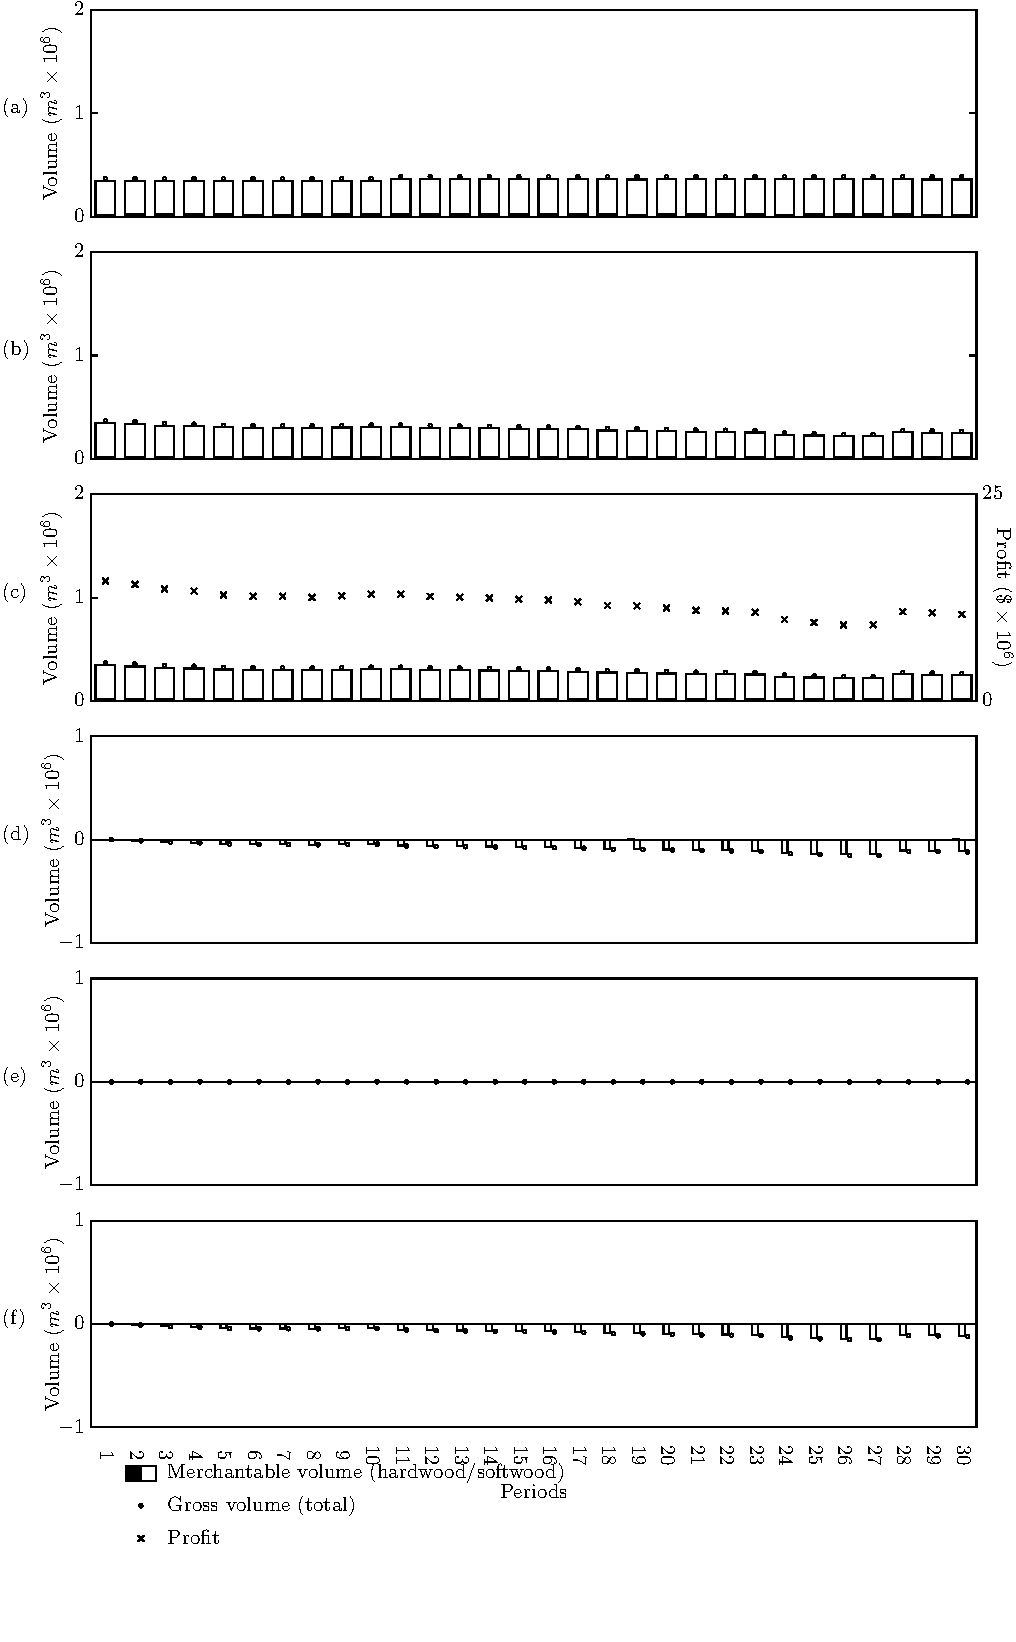
\includegraphics[width=10cm]{images/appendix/s6-1_p30a01}
%   \caption{Base bilevel scenario (same as Scenario 1 presented in Chapter 2).}
%   \label{fig:scenario_bilevel-base}
% \end{figure}

% Some series contain a large number of scenarios. In some cases we present only summary results here, with more detailed simulation results relegated to appendix. Table \ref{tab:scenario_series} summarizes scenario series, with references to appendices.

% \begin{table}
%   \centering
%   \begin{tabular}{lll}
%     \hline
%     Scenario Series Description & Section Reference & Appendix Reference \\
%     \hline
%     Relaxation of line-wise profitability constraint & \S\ref{sec:scenario_series_0} & Appendix \ref{ap:scenario_series_0} \\
%     Varying planning horizon length & \S\ref{sec:scenario_series_0} & Appendix \ref{ap:scenario_series_1} \\
%     %2 & Varying end-product prices & \S\ref{sec:scenario_series_2} & Appendix \ref{ap:scenario_series_2} \\
%     %3 & Varying end-product prices & \S\ref{sec:scenario_series_3} & Appendix \ref{ap:scenario_series_3} \\
%     Varying softwood AAC attribution & \S\ref{sec:scenario_series_4} & Appendix \ref{ap:scenario_series_4} \\
%     Varying tightness of even-flow constraints & \S\ref{sec:scenario_series_5} & Appendix \ref{ap:scenario_series_5} \\
%     \hline
%   \end{tabular}
%   \caption{Description of scenarios in series 6-4.}
%   \label{tab:scenario_series}
% \end{table}

\section{Varying Softwood AAC Attribution}
\label{sec:scenario_series_4}

This scenario series tests the effect of varying the proportion of softwood AAC that the principal attributes to the agent in each planning cycle. This series has a direct potential application to real-world cases; the principal controls the wood supply, and is not obligated to allocate 100\% AAC to timber licencees\footnote{For example, provincial governments policy on Crown forest in Canada typically holds back a small fraction of AAC (around 5\%) with generally vague justification that this hold-back policy satisfies the need for some form of safety buffer in the wood supply.}.

We use a shorthand notation to refer to particular scenarios (e.g., \emph{hw100sw110} refers to the scenario with 100\% of hardwood AAC allocated and 110\% of softwood AAC allocated).
Scenario hw100sw100 corresponds to our reference scenario (i.e., 100\% attribution of both hardwood and softwood AAC). 
We simulate six alternate AAC allocation levels (110\%, 105\%, 95\%, 90\%, 80\%, 60\%. 

As might be expected based on results presented in Chapter 1, over-allocating softwood AAC (i.e., scenarios hw100sw110 and hw100sw105) has a negative effect on long-term wood supply, with wood supply stability deteriorating as a function of over-allocation. However, the effect is moderate; we can conclude the bilevel wood supply model is moderately sensitive to AAC allocation level for our test case. 

Wood supply stabilility improves gradually as we continue to reduce allocation down to 60\% of softwood AAC. At the 60\% allocation level, wood supply stability is completely restored. Withholding a large fraction of softwood AAC indirectly creates a form of safety stock, which offsets gradual wood supply decline observed in the reference scenario\footnote{As discussed in Chapter 2, the slow decline in AAC observed in the reference scenario is attributable to the agent planning his own harvest schedule in the second stage of each planning cycle, which results in a slightly different mix of stand types than those featured in the first period of the optimal wood supply solution. The (deterministic) optimal wood supply solution, being located in an extreme point of feasible solution space, is highly prone to infeasibility, and sensitive to deviations from the optimal solution.}. 

\begin{figure}[H]
  \centering
  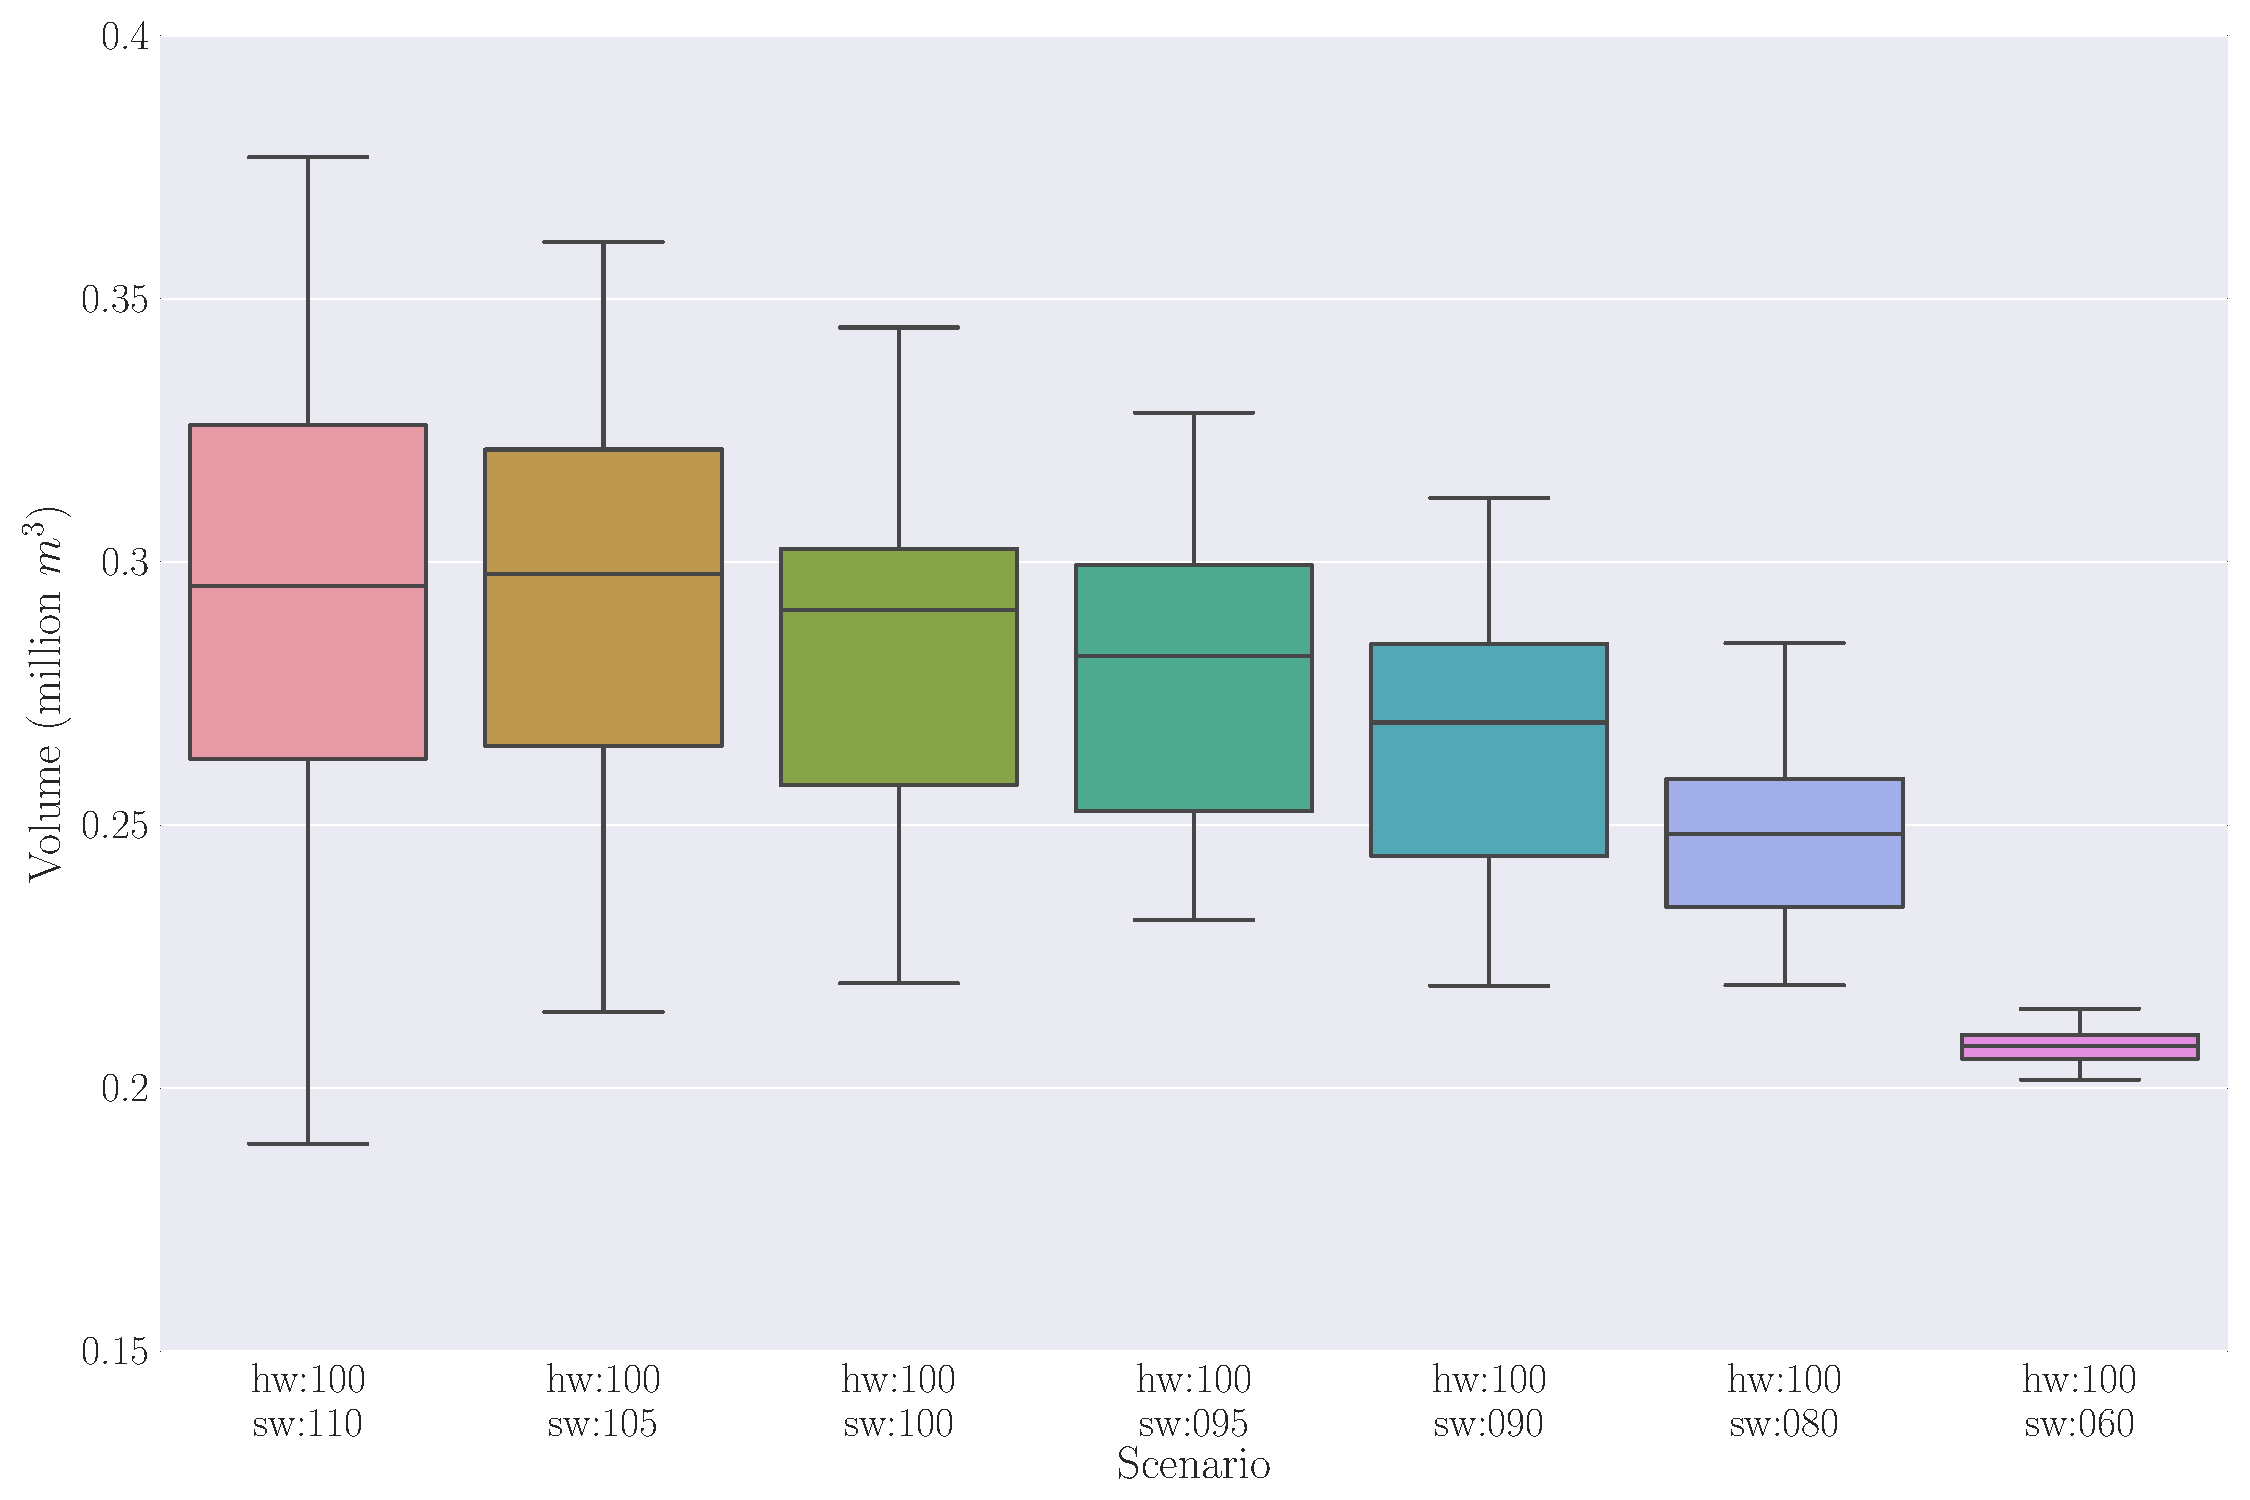
\includegraphics[height=10cm]{images/boxplots_series4}
  \caption{Wood supply stability for a range of softwood AAC attribution levels. }
  \label{fig:scenario_series_4}
\end{figure}

\section{Varying Planning Horizon Length}
\label{sec:scenario_series_1}

This scenario series tests the impact of varying planning horizon length for both principal and agent. 
We test all combinations of horizon lengths for values 30, 20, 10, 5,  and 1 periods. 
Agent horizon is never allowed to be longer than principal horizon, which leaves 15 valid horizon length combinations.
We use a shorthand notation to refer to particular scenarios (e.g., \emph{p30a01} refers to the scenario with a 30-period principal horizon and a 1-period agent horizon).
Scenario p30a01 is our reference scenario for this series, and corresponds to the \emph{status quo} horizon lengths used in Quebec today.
Simulation results reveal interesting patterns on two levels.

%Detailed simulation results are presented in Appendix \ref{ap:scenario_series_1}.

On the first level, longer planning horizons improve stability of long-term wood supply. This effect is most pronounced when comparing scenarios with matched principal and agent horizon lengths (i.e., scenarios p30a30, p20a20, p10a10, p05a05, p01a01). This supports the common belief that long modelling horizons help stabilise solutions from long-term wood supply models (although we use a bilevel wood supply model here, which is not common practice).

One the second level, relative effect of principal horizon length on wood supply stability becomes gradually less pronounced as agent horizon shortens, with the least effect observed for single-period agent horizons. For example, shortening principal horizon length in the reference scenario from 30 to 10 periods (i.e., scenarios p30a01, p20a01, p10a01), has relatively little impact on wood supply. This would indicate that the destabilising effect of short agent planning horizon (due to residual systematic drift that is not anticipated by the bilevel model) overwhelms the stabilising effect of lengthening principal horizon. 

If one focuses on the p30 scenarios (i.e., p30a01, p30a05, p30a10, p30a20, p30a30), results provide some insight into the opportunity cost (in terms of both the magnitude and stability of long-term fibre supply) of maintaining the \emph{status quo} distributed wood supply planning process, where a relatively short-sighted agent is responsible for final implementation of harvesting operations. 

There is a parallel here with the \emph{price of anarchy} concept in game theory \citep{shoham2009multiagent, nisan2007algorithmic}. The contrast between reference scenario p30a01 and best-case scenario p30a30 can be interpreted as an upper-bound estimate of the price of maintaining the \emph{distributed} nature of the wood supply planning process (i.e., allowing the agent to plan his own harvesting, relative to a scenario where the principal controls both long-term wood supply planning and short-term fibre procurement planning processes). 

We specify that this is an \emph{upper bound} estimate, as scenario p30a30 makes rather optimistic assumptions regarding the ability of the principal to produce long- and short-term feasible fibre procurement plans using a simple two-stage planning process as simulated here. Recall that we present simulation results from highly aggregated models. In practice, as-implemented fibre procurement plans are the end product of a complex hierarchical planning process, which iteratively refines plans until they are operationally feasible. Much of the detailed information required to efficiently produce feasible fibre procurement plans is absent from the high-level simulations we present here. To preserve both long- and short-term feasibility, the two-stage planning process (as simulated here) would have to be extended to include an \emph{iterative} dimension; the long-term plan would have to be iteratively constrained, based on feasibility feedback from the (disaggregated) short-term planning level, until the first period of the long-term plan converges with the short-term plan. The process of iterativly constraining the long-term wood supply plan would have either a null (best-case) or negative effect on final AAC, hence our qualification of the contrast between scenarios p30a30 and p30a01 as an \emph{upper bound} estimate of the price of distributed wood supply planning.

In practice, the agent (i.e., the industrial fibre consumer) has both the motivation and the technical expertise required to plan and implement economically efficient short-term fibre procurement plans. It is not clear that the principal has either the proper motivation or the technical capability (recall the information assymmetry that induces the principal-agent problem in the first place) to take over short-term fibre procurement planning (i.e., become an industrial fibre supplier, rather than simply a steward of the public forest resource) without negatively affecting industrial profitability (i.e., stability of fibre cost and value-creation potential). Given the tight profit margins typical of the forest products industry in many jurisdictions, it seems unlikely that the principal could completely exclude the agent from the fibre procurement planning process without destabilising economic sustainability of the forest industry.

Simulation results suggest that the principal could improve long-term wood supply stability by inciting the agent to adopt a longer planning horizon. The case where principal and agent horizon lengths are equal is equivalent to the principal subsuming the agent (i.e., principal has total control of fibre procurement activities, including final selection of stands to be harvested). Note that we simulate perfect anticipation of agent behaviour, thus our simulations results represent optimistic upper bounds potential wood supply. In reality, the principal has limited power to incite the agent to extend his planning horizon beyond one period, so forcing an extension of the agent's planning horizon in the bilevel anticipation may in fact introduce a problematic bias. Development of such incentive policies, using game-theoretic analysis of the decoupling point between principal and agent and the \emph{price of anarchy} concept, represents an interesting direction for futher research.

Note that computational effort required to solve wood supply models can increase exponentially with the number of planning periods for certain model formulations, mostly due to combinatorial explosion of potential future system states for large numbers of planning periods. Our test wood supply model solves very quickly (i.e., approximately 10 seconds), in part due to the efficient SilviLab solver engine, however production models using commercial wood supply modelling software (e.g., Remsoft Woodstock) may require significantly more computational effort to solve similarly-size instances. These long solution times may limit the number of scenarios that can realistically be run by government wood supply analysts, which may in turn limit the quality and scope of wood supply analyses. Our simulation results hint at a potentially interesting tradeoff between computational effort and solution quality. For our test case, principal planning horizon can be shortened by a factor of 3 (i.e., from 30 to 10 periods) with minimal effect on wood supply stability\footnote{We suspect that the amount of planning horizon compression that the principal can safely implement, without inducing unacceptable increase in risk of wood supply failure, is linked to a number of factors that will vary between problem instances (e.g., timing of the critical period and, tightness of even-flow-constraints, etc.).}. Exploratory wood supply scenarios, or sensitivity analyses requiring large numbers of simulations, could potentially be run using shortened model horizons; assuming limited budget for wood supply analysis resources, there is potential to either reduce the cost of analysis with minimal impact on quality, or to improve the quality of the analysis at similar cost.  

%The second pattern is that long-term wood supply is more stable when principal and agent planning horizon lengths are equal. It is not realistic to expect the agent to spontaneously abandon his 1-period horizon in favour of a 30-period planning horizon. However, our simulation results suggest that the principal could indirectly improve long-term wood supply stability by inciting the agent to adopt a longer planning horizon. Although development of such incentive policies is beyone the scope of this project, this represents an interesting direction for futher research.


\begin{figure}[H]
  \centering
  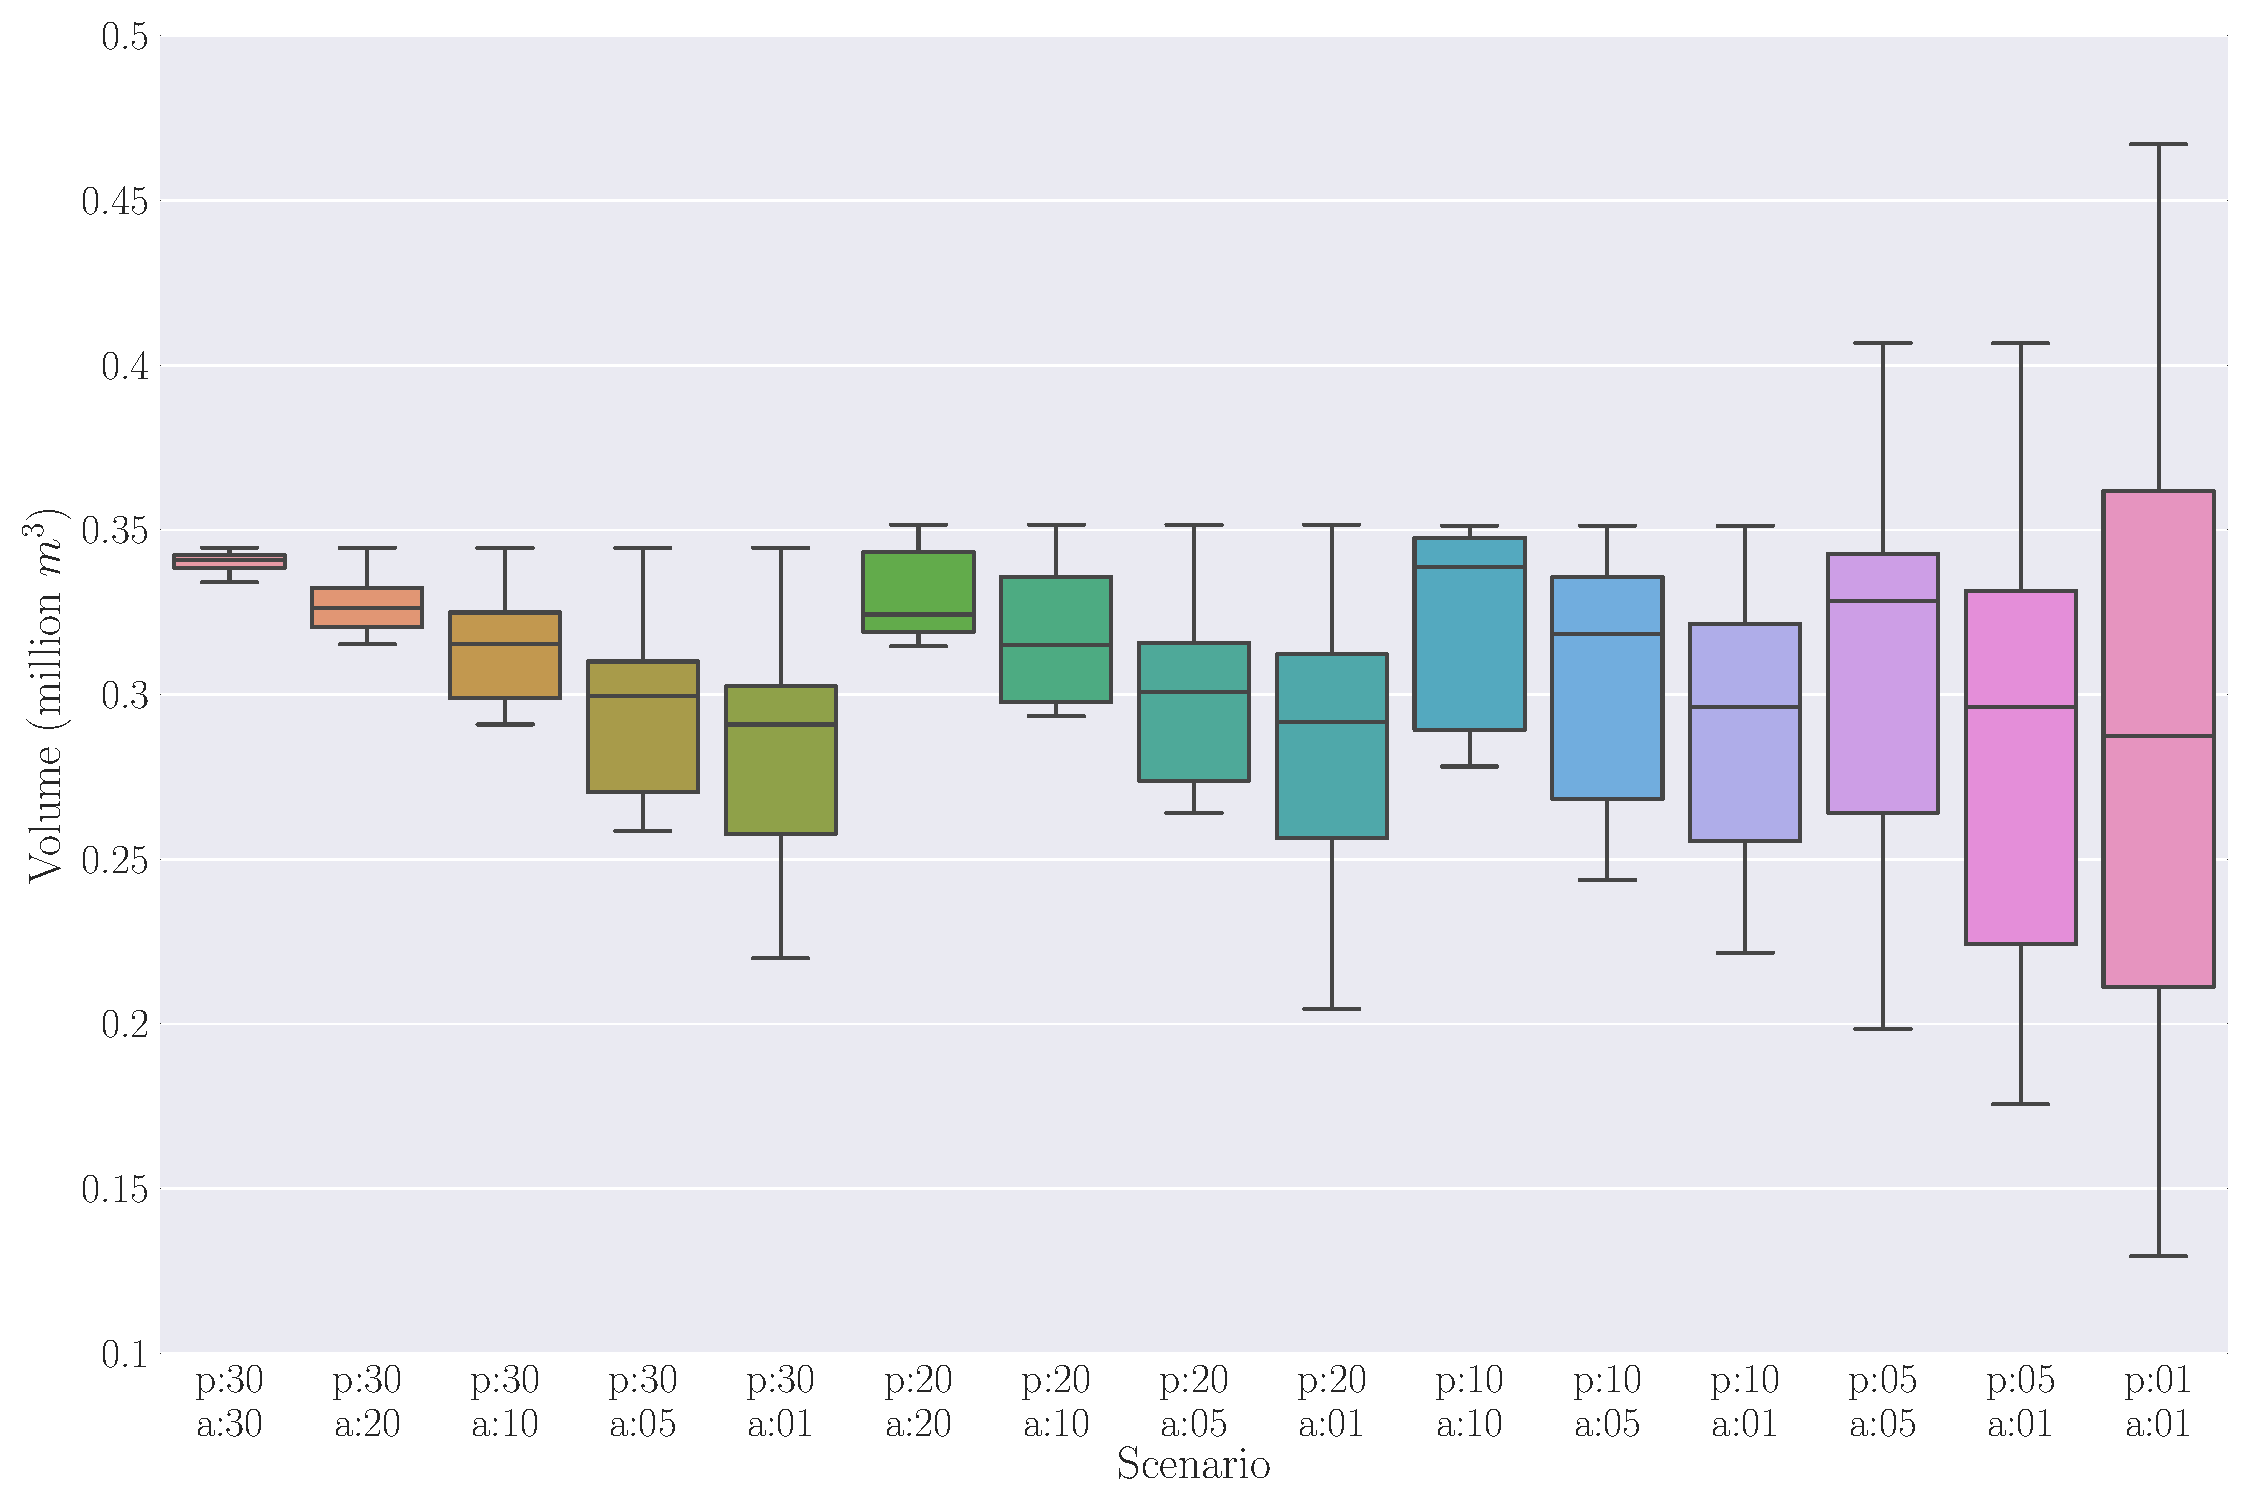
\includegraphics[height=10cm]{images/boxplots_series1}
  \caption{Wood supply stability for a range of combinations of principal and agent planning horizon length. }
  \label{fig:scenario_series_1}
\end{figure}

% \section{Increasing End-product Prices}
% \label{sec:scenario_series_2}

% This scenario series tests the impact of increasing end-product prices in the agent network. We increase all products prices proportionately (i.e., perfectly correlated price increase, relative to reference scenario values), and keep them constant for all 30 iterations. We test ten price scaling factors: 1.6, 2.2, 2.8, 3.4, 4.0, 4.6, 5.3, 5.9, 6.4, and 7.1. 

% We were initially surprised to observe that prices could be scaled by up to 400\% with only negligible effect on agent fibre consumption volume. Further analysis revealed that this is expected behaviour, given the configuration of our test dataset. Low capacity of the single hardwood sawmill is the binding constraint (i.e., bottleneck) for the first five scenarios in this series; the increase in hardwood end-product price is not sufficient to offset the cost of 

% , until prices are scaled by a factor of 4.6, at  which point agent fibre consumption (and profit) increases suddenly 

% \section{Decreasing End-product Prices}
% \label{sec:scenario_series_3}


\section{Varying Tightness of Even-flow Constraints}
\label{sec:scenario_series_5}

This scenario series tests the effect of varying the tightness of even-flow constraints. The reference scenario hw005sw005 simulates a 5\% even-flow constraint gap for both hardwood and softwood. We simulate 5 alternate tighness values (0\%, 1\%, 10\%, 20\%, and 50\%). 
We use a shorthand notation to refer to particular scenarios (e.g., \emph{hw001sw001} refers to the scenario with a 1\% even-flow constraint gap for both hardwood and softwood).

As might be expected, long-term wood supply is more stable when the constraints are tighter, and more variable when the constraints are relaxed. Furthermore, relaxing the even-flow constraints has a negative effect on mean AAC. However, our model is relatively insensitive to this parameter, and remains surprisingly stable with a 50\% even-flow constraint gap. 

\begin{figure}[H]
  \centering
  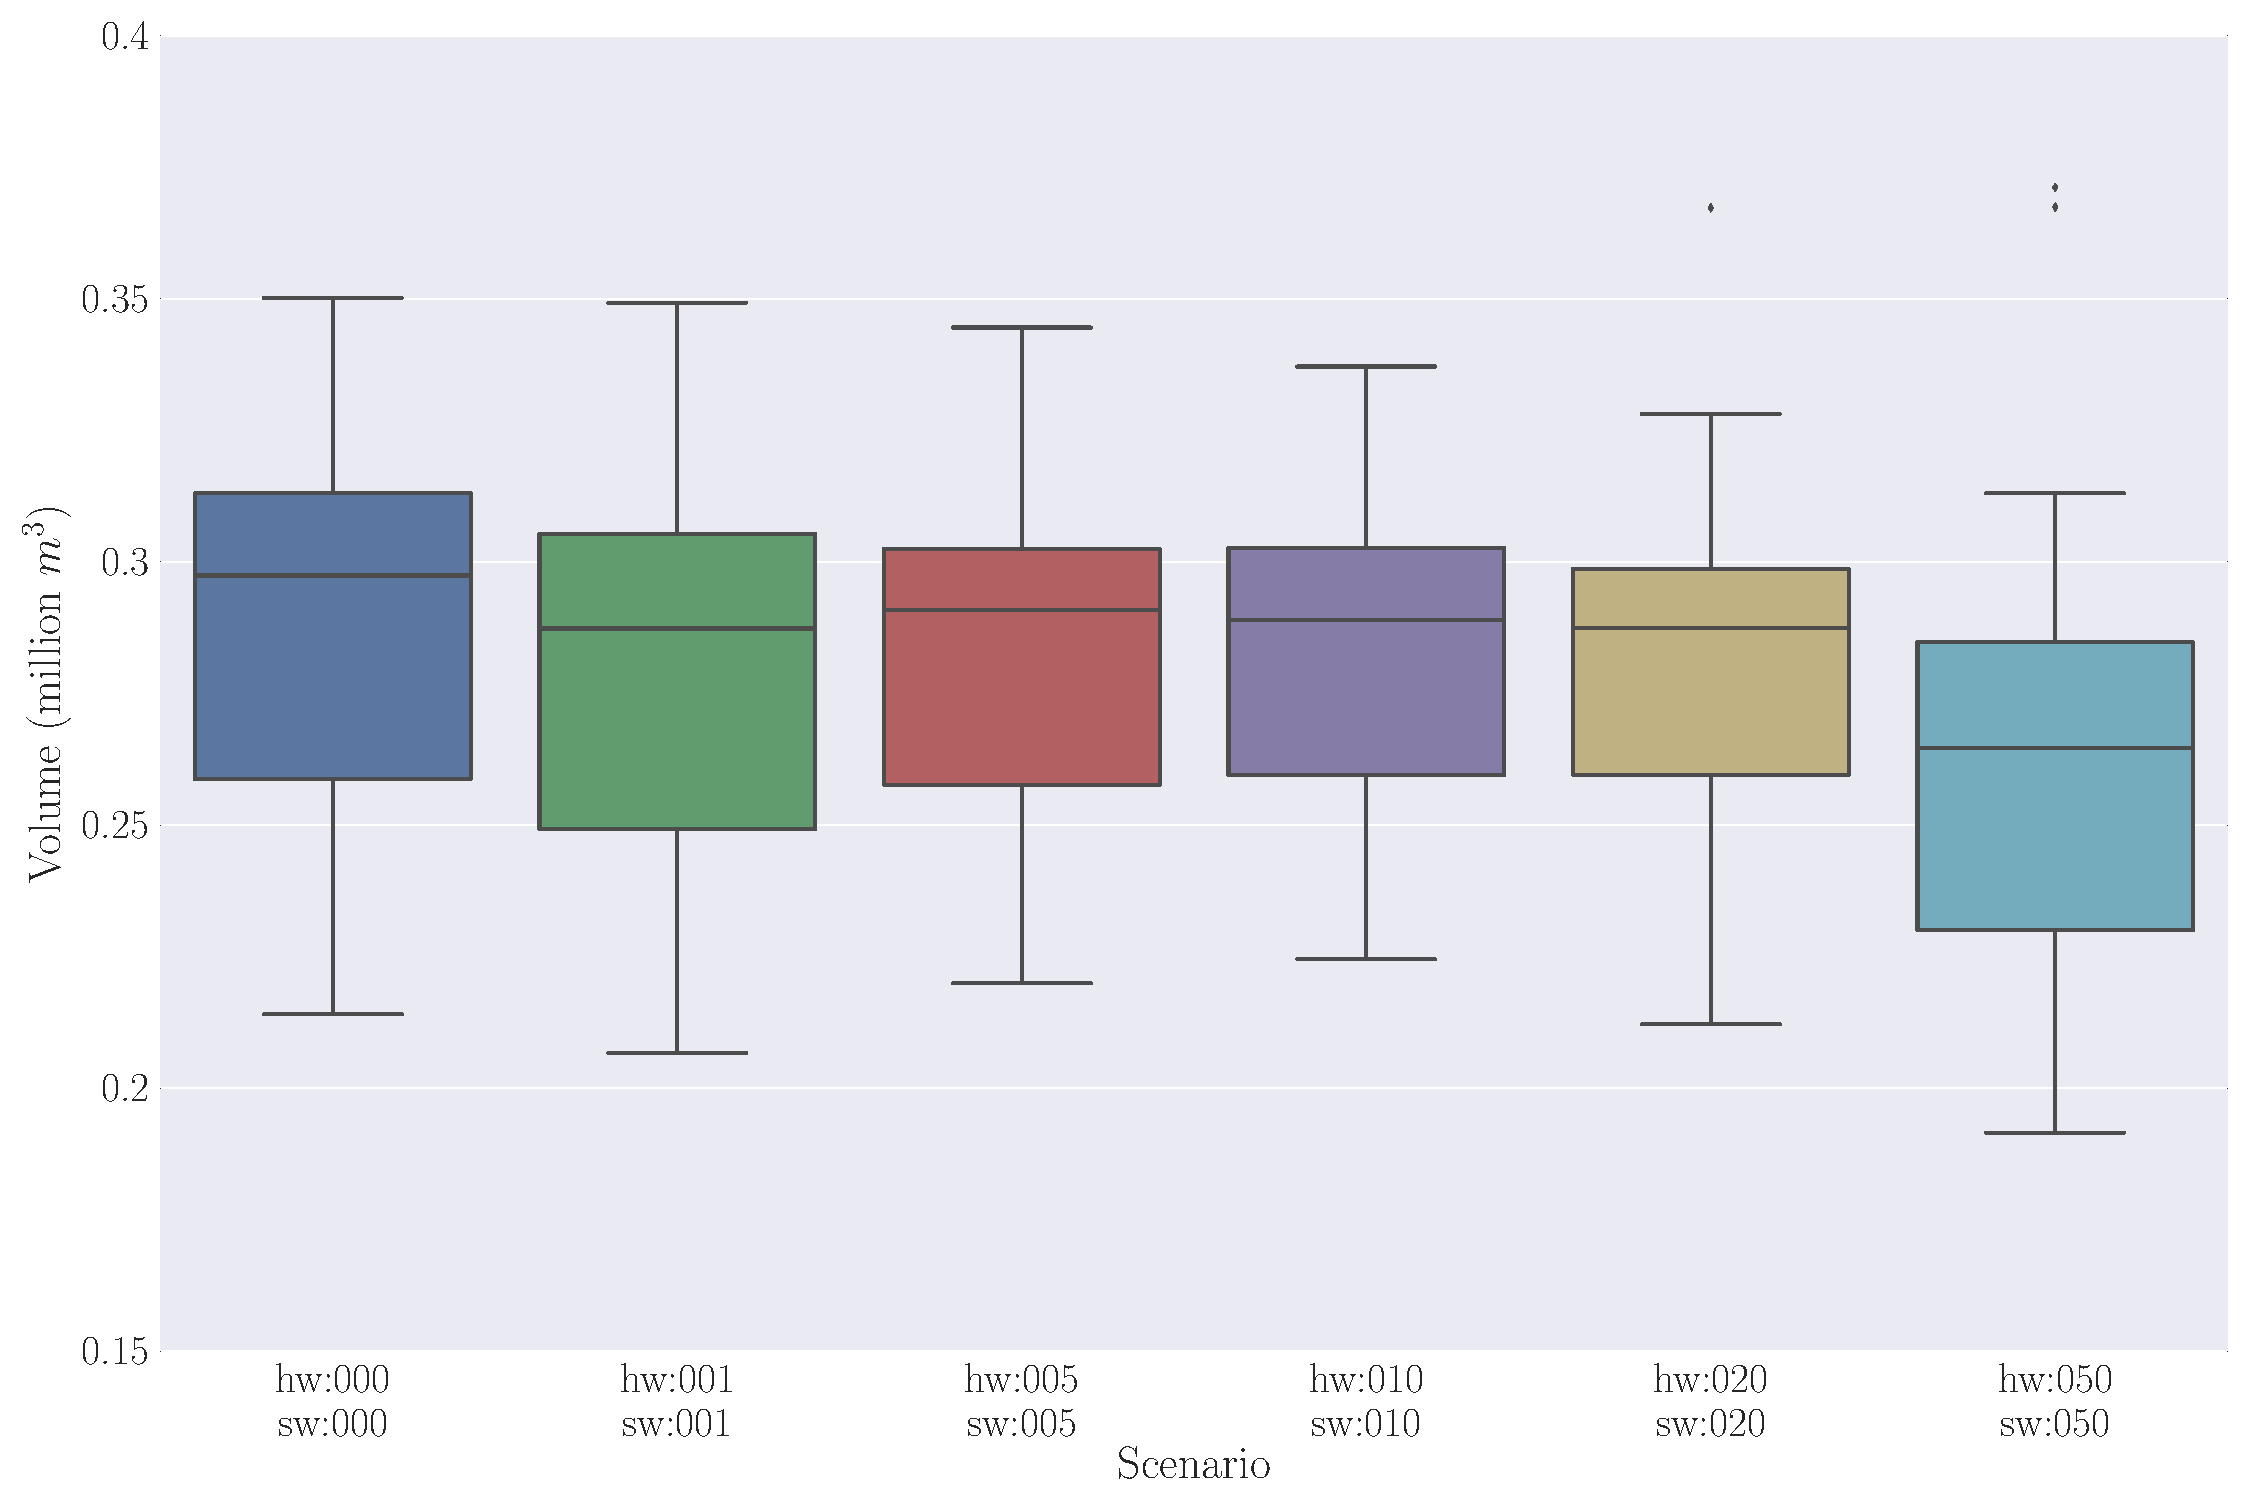
\includegraphics[height=10cm]{images/boxplots_series5}
  \caption{Wood supply stability for a range of even-flow constraint tighness levels. }
  \label{fig:scenario_series_5}
\end{figure}

\section{Stochastic Agent Fibre Demand}
\label{sec:scenario_series_6}

The reference scenario optimistically simulates perfect anticipation of agent fibre consumption volume. In practice, we expect some random error in the principal's anticipation of fibre demand. This scenario series tests the sensitivity of wood supply to controlled stochasticity in actual agent fibre demand.


To implement this scenario series, we simulate randomly-generated AAC consumption levels in the second stage of each planning cycle. More specifically, we randomly generate the proportion of AAC consumed in each cycle by sampling from a uniform distribution on the interval $[0.9, 1.1]$ (i.e., AAC $\pm 10\%$). This is similar to the range and distribution of historic variation in AAC consumption in Canada between 1990 and 2012 (see Figure \ref{fig:aac_consumption}).

Figure \ref{fig:scenario_series_6} presents results from 20 replicates of the experiment, comparing re-planned AAC for the reference (i.e., deterministic) and test (i.e., stochastic) demand scenarios. For the stochastic scenario, we plot the $2\sigma$ error band (i.e., 95\% of expected variability is contained within the error band). 

\begin{figure}[H]
  \centering
  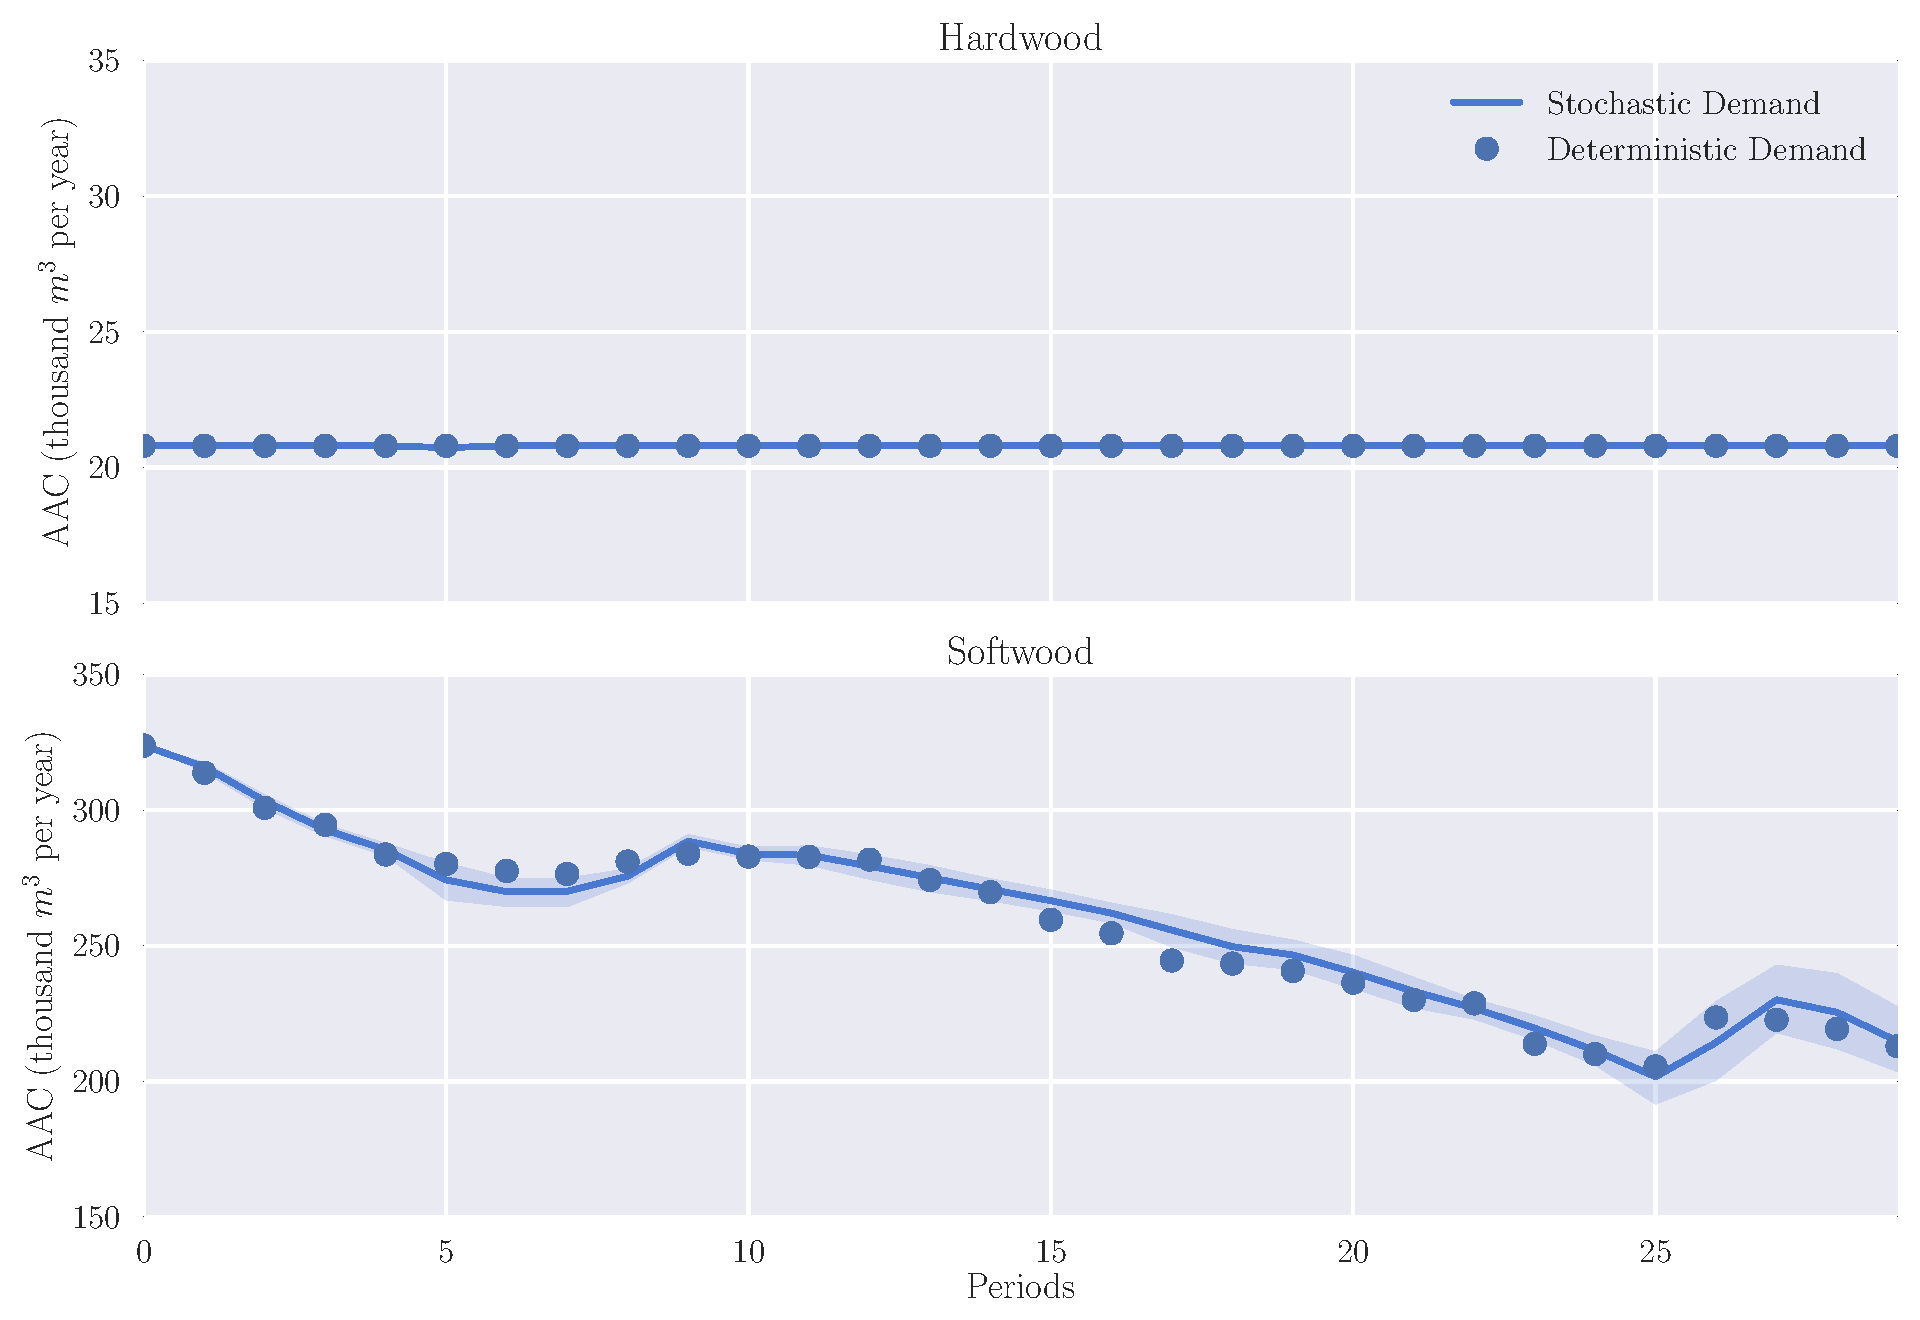
\includegraphics[width=\textwidth]{images/tsplot_2sigma}
  \caption{Comparison of re-planned AAC under deterministic (reference) and stochastic (test) anticipation of AAC consumption.}
  \label{fig:scenario_series_6}
\end{figure}
 
These simulation results show that error in anticipation of demand within the bilevel model is not problematic when actual fibre demand is uniformly distributed on an interval centered on current AAC. This is an important result in terms of potential feasibility of implementing a bilevel wood supply modelling solution in practice; although real-world implementation of the agent-anticipation mechanism will never be perfect (i.e., there will always be residual information asymetry between the principal and the agent), this error many not have a significant effect on long-term wood supply sustainability \emph{as long as it is not biased} (i.e., mean fibre consumption is randomly distributed on an interval centered on AAC).  

These results have an interesting potential policy application. The principal could potentially allow the agent to exceed AAC in periods of peak demand and lag behind AAC in periods of depressed demand. By providing a certain amount of short-term flexibility, this type of policy could potentially allow the agent to improve mean profit, by capturing more short-term value creation opportunities, without compromising sustainability of the wood supply.

\section{Relaxation of Line-wise Profitability Constraint}
\label{sec:scenario_series_0}

%%%%%%%%%%%%%%%%%%%%%%%%%
% Text pasted from article 2:

% Scenario 6 shows the potential benefit of relaxing the agent's line-wise profitability constraint. This simulates a more centralized fibre procurement behaviour in the agent than the standard agent behaviour simulated in scenarios 2 through 5. Scenario 6 allows the agent to maximize the sum of profits from both hardwood and softwood lines. This opens up the possibility for the agent to dispose of excess hardwood fibre supply (at a moderate cost) in order to gain access to significant extra volume of softwood from previously-inaccessible high-hardwood-content mixedwood stands. The cost of disposing of the relatively small volume of excess hardwood fibre is offset by the profits from processing and sale of a relatively large volume of newly-available softwood fibre. 

% This increase in hardwood fibre consumption has a positive-feedback effect on long-term fibre supply; the principal may now harvest the problematic mixedwood stands at a faster in the first few planning cycles. These mixedwood stands (which where left standing in previous scenarios) can now be replaced with pure softwood plantations. In the medium term, this has the effect of partially re-aligning the inventory of standing timber with industrial fibre demand. In practice, agent behaviour more closely resembles the greedy agent bhaviour simulated in scenarios 1 through 6.

% Centralized fibre procurement planning almost double average fibre consumption (92\% increase) relative to scenario 3 (i.e., base bilevel scenario). This significant increase in potential fibre consumption represents an important opportunity of the agent, however implementing intra-agent collaborative fibre procurement behaviour is between the is beyond the control of the principal. There is nonetheless a clear incentive for the principal for lobby the agent to align his fibre consumption capacity with the potential wood supply. 
%%%%%%%%%%%%%%%%%%%%%%%%%%%%%

Our base bilevel scenario imposes a \emph{line-wise profitability} constraint on the agent sub-model. For our test case, we aggregate all fibre flows into the agent model into two product lines (i.e., \emph{hardwood} and \emph{softwood}). The line-wise profitability constraint requires fibre flows from each of these lines to be independently profitable, which  plays an important role in our simulation of wood supply failure in Chapter 1. The line-wise profitability constraint in our agent model reflects a common situation in many real-world value creation networks: hardwood and softwoood mills are independently owned and managed, which affects the species composition of stands that are scheduled for harvest in each planning cycle.  

For our test dataset, hardwood fibre consumption is constrainted by low hardwood fibre processing capacity\footnote{Hardwood logs must pass through a single hardwood sawmill, whose annual processing capacity is limited to approximately one third of initial hardwood AAC.}. Flow conservation constraints in our model limit harvest volume to consumed volume (i.e., all harvested fibre must be consumed). In the reference scenario the combination of low hardwood processing capacity, high softwood fibre demand, line-wise profitability constraints and flow conservation constraints limits sustainable bilevel AAC. 

%To harvest the entire softwood AAC while limiting hardwood fibre harvesting to a fraction of AAC, the stands selected for harvest by the agent (in the second stage of each planning cycle) must feature a higher proportion of softwood than the stands that are schedule for harvest in the first period of the wood supply model solution. The forest stands available for harvesting in future planning cyclces are affected by what was harvested in the current planning cycle. 

%Thus, agent avoidance of hardwood-rich stands in his harvesting plans causes systematic drift of the forest system state: the unharvested hardwood-rich stands form an increasingly large proportion of standing timber inventory. Mature softwood-rich stands grow increasingly scarce at each planning cycle, forcing the agent to reduce his total consumption volume. 

Our test dataset features an alternative agent process that could potentially consume hardwood fibre (besides the single hardwood sawmill), which we will designate the \emph{storage} process. The storage process has a negative net unit value (i.e., the agent has to pay a constant unit cost to push fibre through this process). The line-wise profitability constraints prevent any fibre form flowing through this process in the reference scenario. 

If the line-wise profitability constraints are relaxed in the agent model (i.e., if we simulate centralized agent fibre procurement planning), the cost of pushing fibre through the storage process may be offset by profits from the additional fibre that can be pulled through the softwood line, which in turn would allow the principal to sustainably increase bilevel AAC. 

Figure \ref{fig:scenario_series_0} shows simulation results for a scenario where we relax the line-wise profitability constraints in the agent model.  This simulates perfectly integrated (i.e., collaborative) agent fibre procurement behaviour, and makes it possible for the hardwood line to operate at a net loss if this is profitable for the network as a whole. 

\begin{figure}[H]
  \centering
  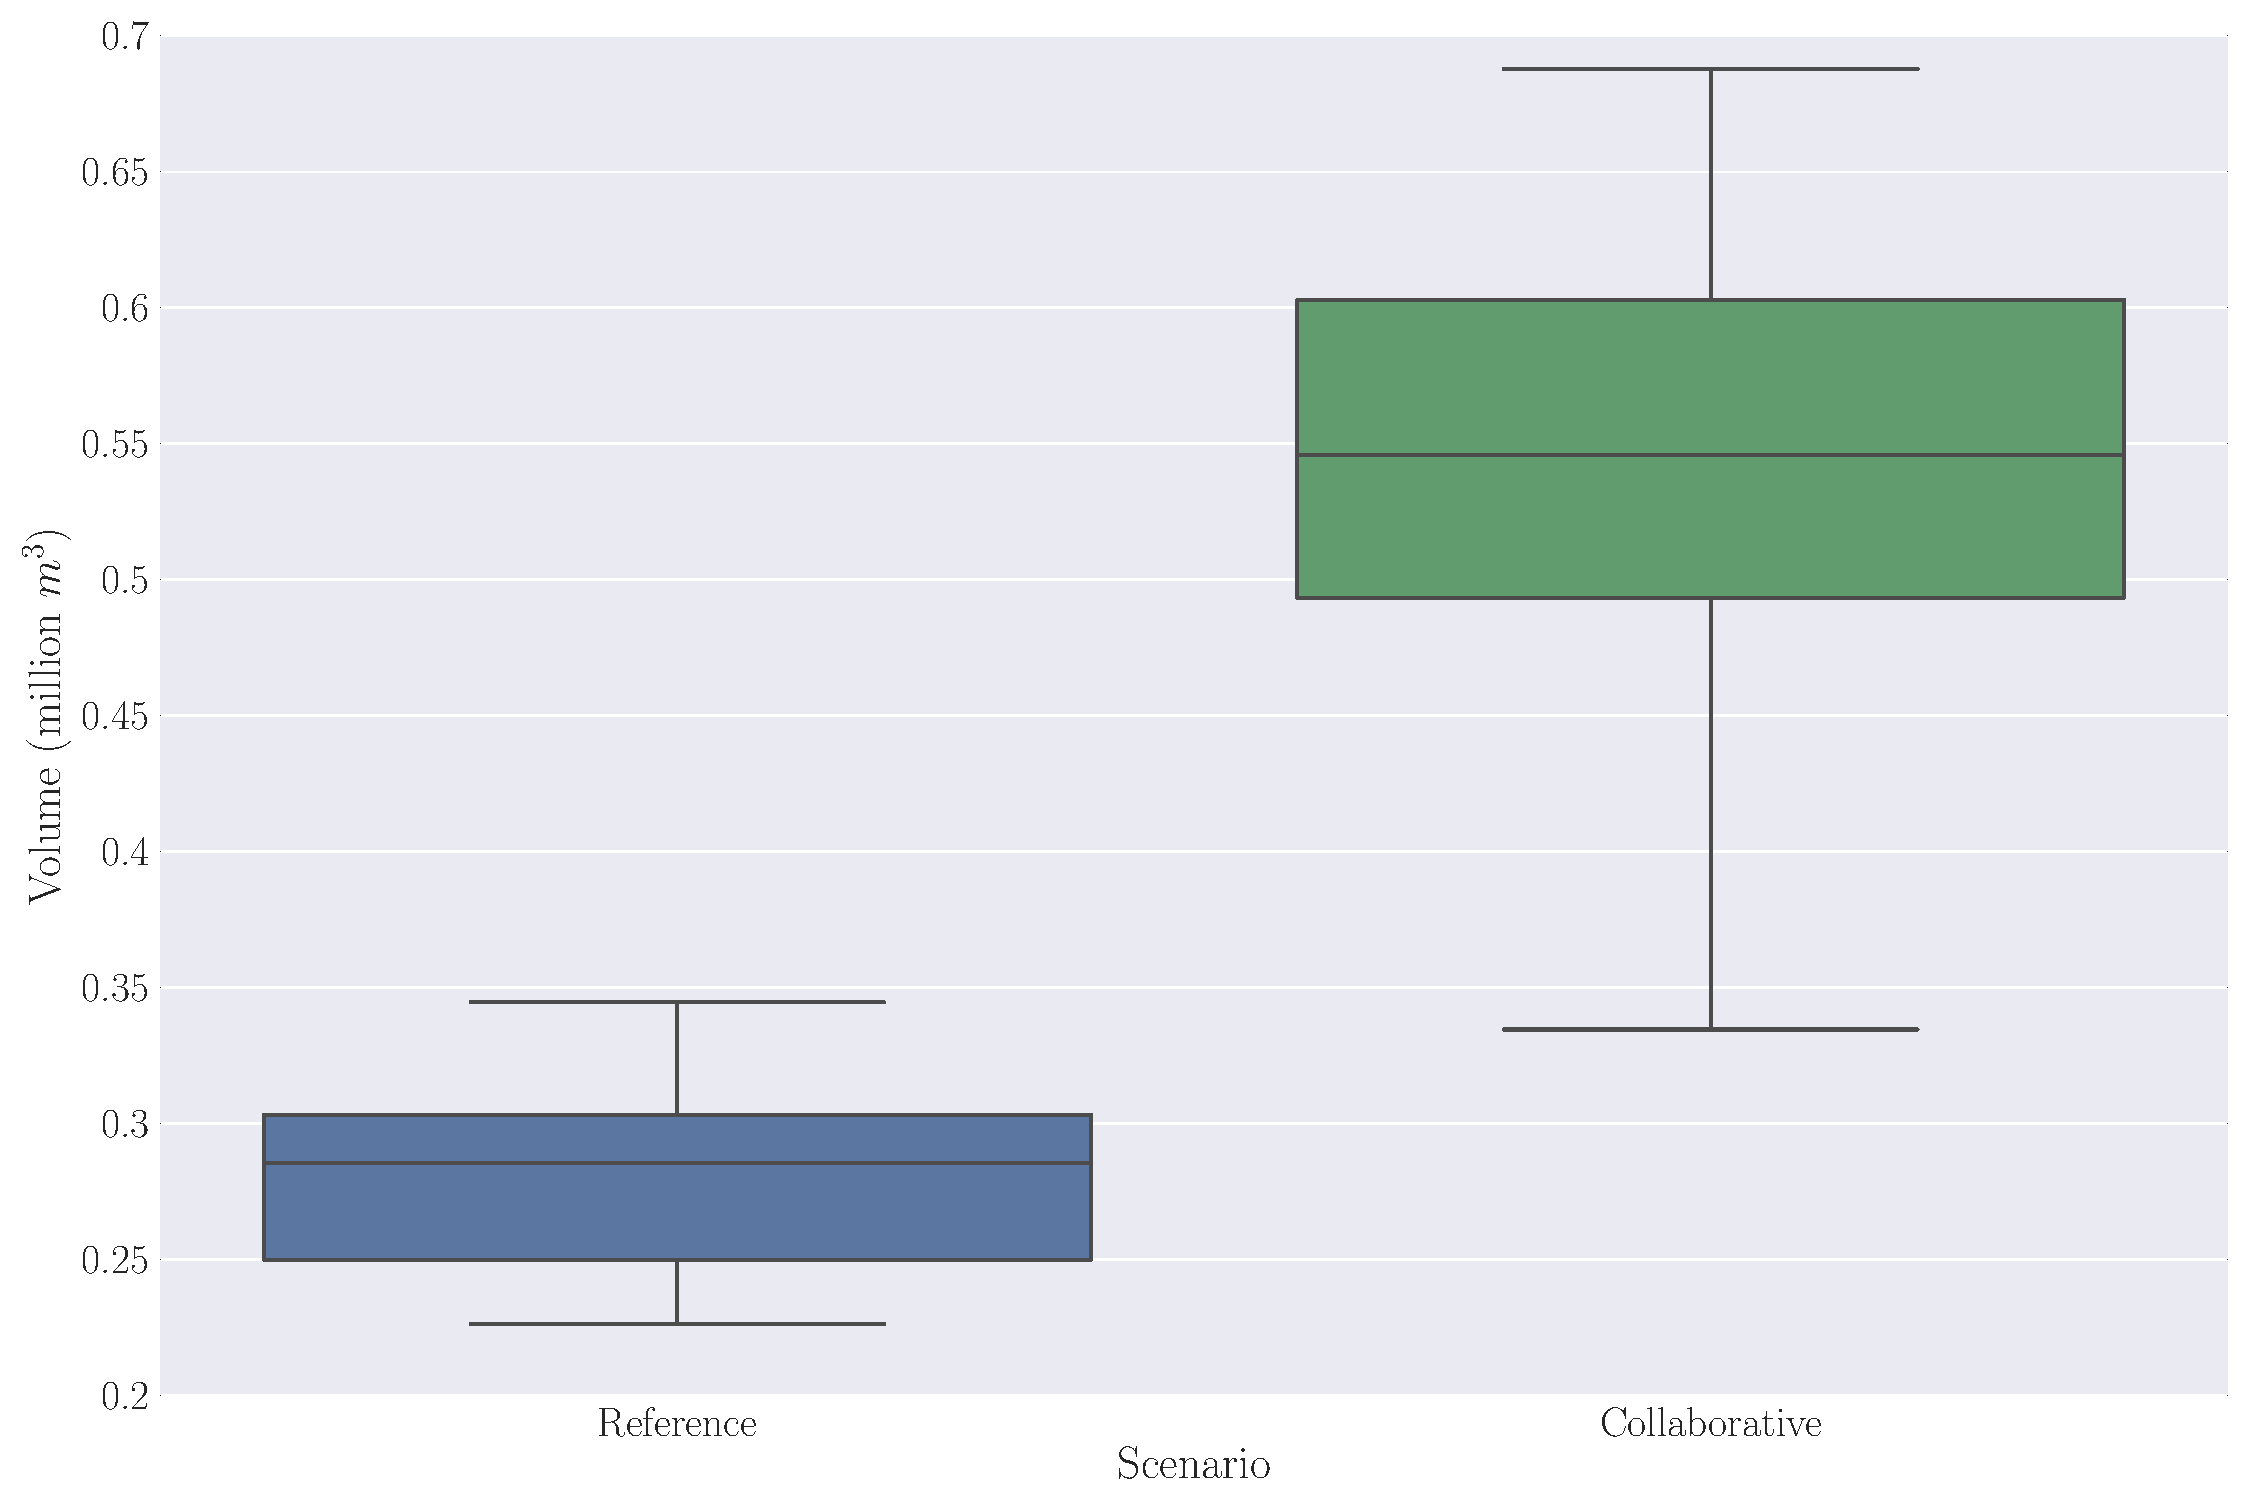
\includegraphics[width=\textwidth]{images/boxplots_series0}
  \caption{Effect of relaxing line-wise profitability constraint (i.e., centralizing agent fibre procurement) on magnitude and stability of wood supply. }
  \label{fig:scenario_series_0}
\end{figure}


% \begin{figure}[h]
%   \centering
%   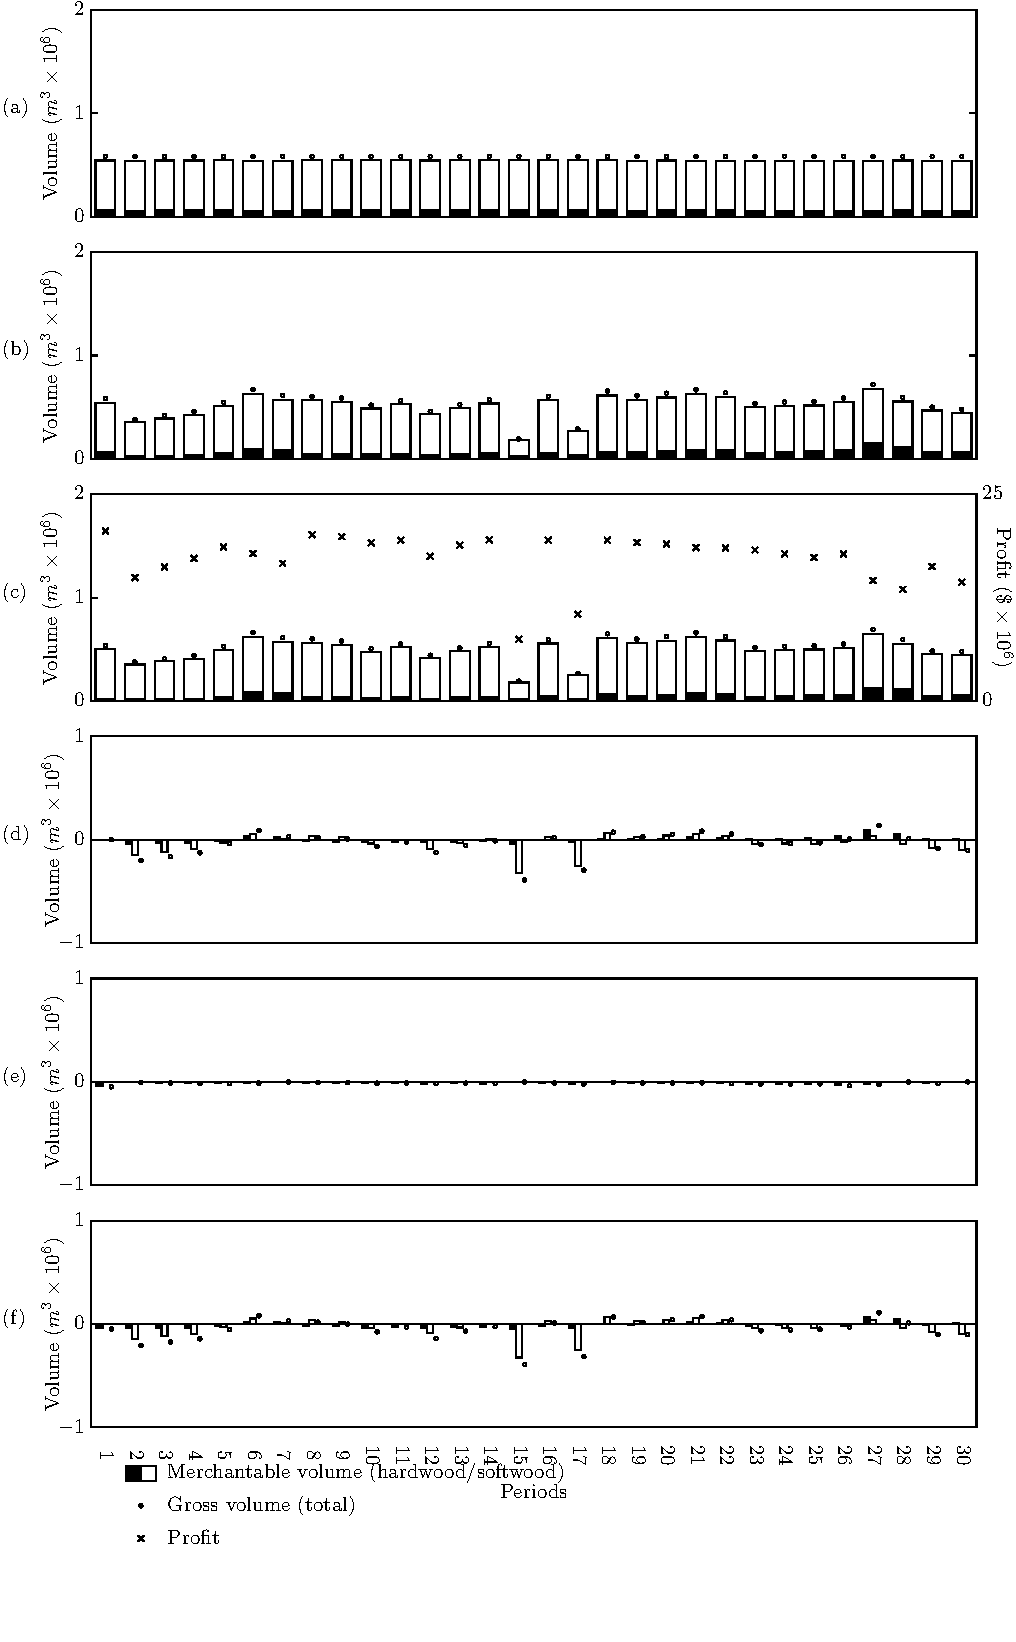
\includegraphics[width=10cm]{images/appendix/s6-6_base}
%   \caption{Scenario simulating relaxed line-wise agent profitability constraint}
%   \label{fig:s6-6_base}
% \end{figure}

\subsection{Benefits and Challenges of Collaborative Fibre Procurement Planning}

Collaborative fibre procurement planning almost double average fibre consumption (92\% increase) relative to the reference scenario. 
%This represents an important opportunity of the agent, however 
Implementing intra-agent collaborative fibre procurement behaviour is beyond direct control of the principal, but he has a clear incentive\footnote{As indicated by the objective function of the wood supply model, which maximizes long-term sustainable fibre consumption.} to lobby the agent to align fibre consumption capacity with potential wood supply. 

For our test case, the increase in hardwood fibre consumption under collaborative fibre procurement planning has a positive-feedback effect on long-term fibre supply. The principal may now harvest the problematic mixedwood stands in the first few planning cycles. These mixedwood stands, which are left standing in the reference scenario, can now be replaced with pure softwood plantations. In the medium term, this has the effect of partially re-aligning the inventory of standing timber with industrial fibre demand. In practice, agent behaviour more closely resembles the greedy agent behaviour simulated in the reference scenario.

The collaborative scenario simulates willingness of the hardwood line to operate at a net loss to benefit the rest of the network.
Some form of collaborative benefit-sharing agreement would have to been in place for this setup to be economically viable for the hardwood sub-agent. Although the potential for collaborative benefit-sharing has been discussed in the litterature, for forestry and other supply-chain contexts \citep{audy2012framework, lehoux2011collaboration, forget2008collaborative, dudek2005negotiation, frisk2010cost, guan2011study, beaudoin2010negotiation}, collaborative fibre procurement planning has received relatively little attention. 
Furthermore, collaborative benefit-sharing fibre procurement agreements in a distributed planning environment seem to be rare, and evidence of such is mostly annecdotal.
Elaboration of benefit-sharing agreements to help balance asymmetrical species-wise fibre demand, and the game-theoretic conditions under which these agreements might be stable, represents a promising direction for further research. 

Simulation of collaborative fibre procurement planning allows the principal to increase bilevel AAC, and brings fibre consumption levels closer to the maximum sustainable level that can be sustained by anticipated forest growth. Wood supply for the collaborative scenario is relatively volatile, tending to jump up and down in a pattern that is not predicted the bilevel wood supply model. This contrasts the slow and steady decline of wood supply in the reference scenario. Both scenarios make similarly optimistic assumptions regarding the ability of the principal to anticipate agent behaviour (i.e., perfect anticipation of fibre consumption \emph{volume}, although agent may select an unanticipated mix of forest types in his harvest plan executed in the second stage of the simulation at each planning cycle). 

We conjecture that the aforementionned volatility could be mitigated by extending the formulation of the bilevel model to include some form of safety-stock management mecanism. Development of an efficient safety-stock management mecanism, and determination of minimal standing timber buffer levels required to stabilize wood supply under fibre demand uncertainty, represent promising topics for further development.


\section{Conclusion}

Using our two-stage rolling-horizon re-planning simulation framework, we tested the sensitivity of the bilevel wood supply model to five different factors. For each factor, we simulate a range of values, which we group into \emph{scenario series}. 

The first scenario series (see \S\ref{sec:scenario_series_4}) tests the effect of varying the proportion of softwood AAC that is attributed to the agent at each planning cycle. Results show that long-term wood supply is more stable at lower attribution levels. The last scenario in this series completely restores wood supply stability, but requires a 40\% reduction of softwood AAC relative to the reference scenario. 

The second scenario series (see \S\ref{sec:scenario_series_1}) examines the relationship between principal and agent planning horizon lengths and long-term wood supply. Results show that longer planning horizons tend to improve both magnitude and stability of wood supply. Conversely, wood supply magnitude and stability tends to degrade as a function of the difference in principal and agent horizon lengths; for a given principal horizon length, the lowest mean wood supply and highest wood supply variability are observed for single-period agent planning horizon. For the reference scenario (i.e., principal plans on 30-period horizon and agent plans on 1-period horizon), some of the potential benefit of the principal forecasting wood supply 30 periods ahead is lost when the agent replans harvesting using on a 1-period horizon. 


% can be almost completely stabilised if softwood attribution is reduced to 60\% of AAC. This is the only distributed wood supply planning scenario we simulate that completely eliminates the systematic drift effect (i.e., wood supply does not decline over time); this is a significant, as it shows that our bilevel model is capable of restoring sustainability to the distributed wood supply planning problem, albeit at the expense of rather dramatic reduction in short-term AAC compared to current practice. Reducing attribution levels is an indirect way of creating a safety stock of standing timber at the critical period. Using more direct modelling approaches to manage this safety stock (as discussed in \citet{raulier2014increasing}), it may be possible to achieve similar wood supply stability at higher consumption levels. 

The third scenario series (see \S\ref{sec:scenario_series_5}) varies the tightness of even-flow constraints. We conclude that varying even-flow constraint gap tightness between 0\% and 50\% has a negative effect on wood supply magnitude and stability, although the effect is surprisingly moderate for our test case.

The fourth scenario series (see \S\ref{sec:scenario_series_6}) tests the effect of adding stochastic variability in fibre demand in the second stage of the simulation at each planning cycle. We conclude that allowing actual fibre consumption to vary in a bounded range on either side of AAC does not necessarily compromise sustainability. This is a promising area for further research, as allowing agent fibre consumption to occasionally exceed AAC (e.g., when markets conditions are favourable) could capture ephemeral value creation opportunities, thereby improving mean profitabilty.

The fifth scenario series (see \S\ref{sec:scenario_series_0}) shows that wood supply in the reference scenario is bound by the line-wise profitability constraint. For our test case, bilevel wood supply could potentially be doubled if the agent adopts more collaborative fibre-procurement behaviour. Assuming that wood supply scarcity is a problem in certain regions, collaborative agent fibre procurement represents a very promising topic for further study.

%\section{Conclusion}
%\label{sec:conclusion3}

The simulation results presented in this chapter provides valuable insight into the performance of the bilevelmodel in a rolling-horizon replanning context. Although the bilevel model clearly helps to stabilise the long-term wood supply\footnote{See Chapter 2 for an in-depth comparison of long-term performance of classic and bilevel models.}, most bilevel scenarios exhibit some form of residual systematic drift (i.e., gradual decline of wood supply at each replanning cycle). The residual drift is moderate, compared to the highly unstable \emph{status quo} scenario (see Figure \ref{fig:scenarios}, scenarios 1 and 3), but a systematic decline in long-term wood supply is nonetheless incoherent with the even-flow constraints in the wood supply model. 

Although wood supply decline for the reference scenario is moderate (approximately 1.3\% decline per planning cycle), the cumulative result after 30 planning cyclse is a 40\% decline in initial wood supply. This decline is not predicted by the bilevel model in any of the 30 cycles of rolling-horizon replanning. We were able to simulate drift-free scenarios in two stable cases: the first scenario in \S\ref{sec:scenario_series_1} (see Figure \ref{fig:scenario_series_1}, scenario p30a30), and last scenario in \S\ref{sec:scenario_series_4} (see Figure \ref{fig:scenario_series_4}, scenario hw100sw060). 

In the first stable case (scenario p30a30 in series 1), we eliminated the residual drift by lengthening agent planning horizon to 30 periods (to match principal planning horizon). 
%Technically, this forces agent behaviour at each planning cycle to more closely match the first-period solution from the principal's optimization model, with eliminates most of the residual incoherence between principal and agent plans. 
Conceptually, this is equivalent to the principal shifting the decoupling point downstream and taking over responsibility for harvest planning (i.e., the principal now controls both first and second stages of the simulation at each planning cycle).
Interestingly, a similar shift in the decoupling point between the principal and the agent was recently implemented in Quebec during a major reform of Crown forest tenure rules \citep{quebec2011loi}. 
However, the scenario we simulate here does not accurately model the new tenure system in Quebec, as it optimistically forces the agent to adopt an artificially long planning horizon. 
In reality, the principal does not have the leverage required to force the agent to lengthen his planning horizon. 
Furthermore, implementing optimistic assumptions regarding agent behaviour into the bilevel model is irrational (recall that the motivation for delevoping the bilevel model in the first place was to mitigate the adverse effects of optimistic asssumptions implicitly embedded into classic wood supply model).
Accurately modelling the new Quebec tenure system within our rolling-horizon simulation framework represents an interesting direction for further development.

In the second stable case (scenario hw100sw060 in series 2), we eliminated residual drift by reducing softwood attribution to 60\% of AAC. This indirectly creates a safety stock in the standing timber inventory that is sufficiently large to compensate for the residual error in agent behaviour anticipation\footnote{Although we simulate perfect anticipation of fibre consumption \emph{volume}, the agent plans his own harvest schedule and tends to select a slighly different mix of forest types than that which was anticipated in the bilevel model. The bilevel model solves a deterministic optimization problem, and even slight perturbations can induce partial infeasibility.}. This scenario shows that safety stock management represents a promising solution to the residual drift problem. \citet{raulier2014increasing} compare performance of direct and indirect safety stock management to mitigate forest fire risk in a wood supply model, and simulate highter AAC under direct safety stock management. We conjecture that a direct safety stock modelling approach could be implemented to more efficiently stabilise the bilevel wood supply model, while maintaining higher sustainable fibre consumption levels than those simulated here in scenario hw100sw060.